\documentclass[french]{article}
\usepackage[T1]{fontenc}
\usepackage[utf8]{inputenc}
\usepackage{lmodern}
\usepackage[a4paper]{geometry}
\usepackage[spanish]{babel}
\usepackage{graphicx}
\title{Resolución de los problemas sobre el archivo "Seno.tex"}
\author{David Alonso Garduño Granados}
\begin{document}
	\maketitle
	
Al inicio los errores que me manda era sobre el paquete "pgfplots":

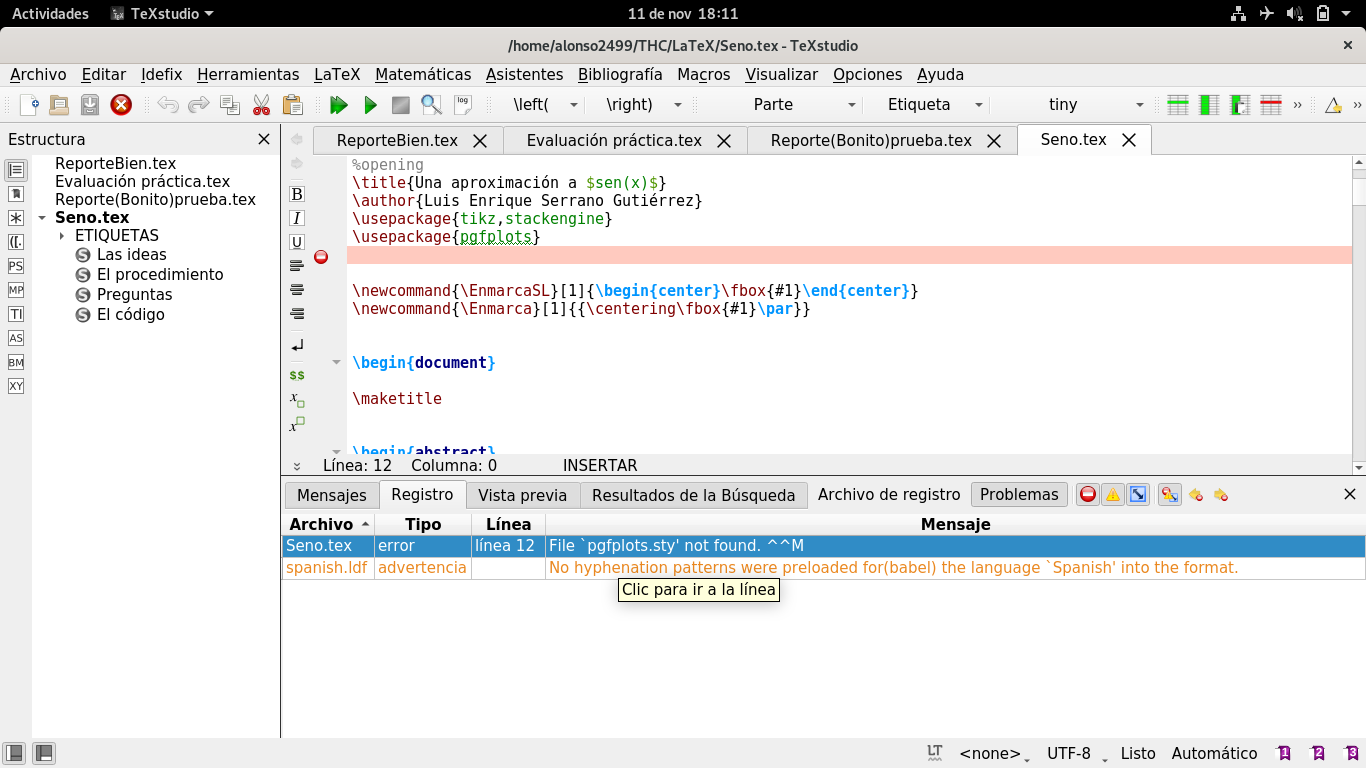
\includegraphics[scale=0.20]{/home/alonso2499/THC/LaTeX/Imagenes/ER4.png} 

Después de esto, esperaba que como el documento anterior fuera el único error que me marcase, así que recurrí a su inmediata instalación:

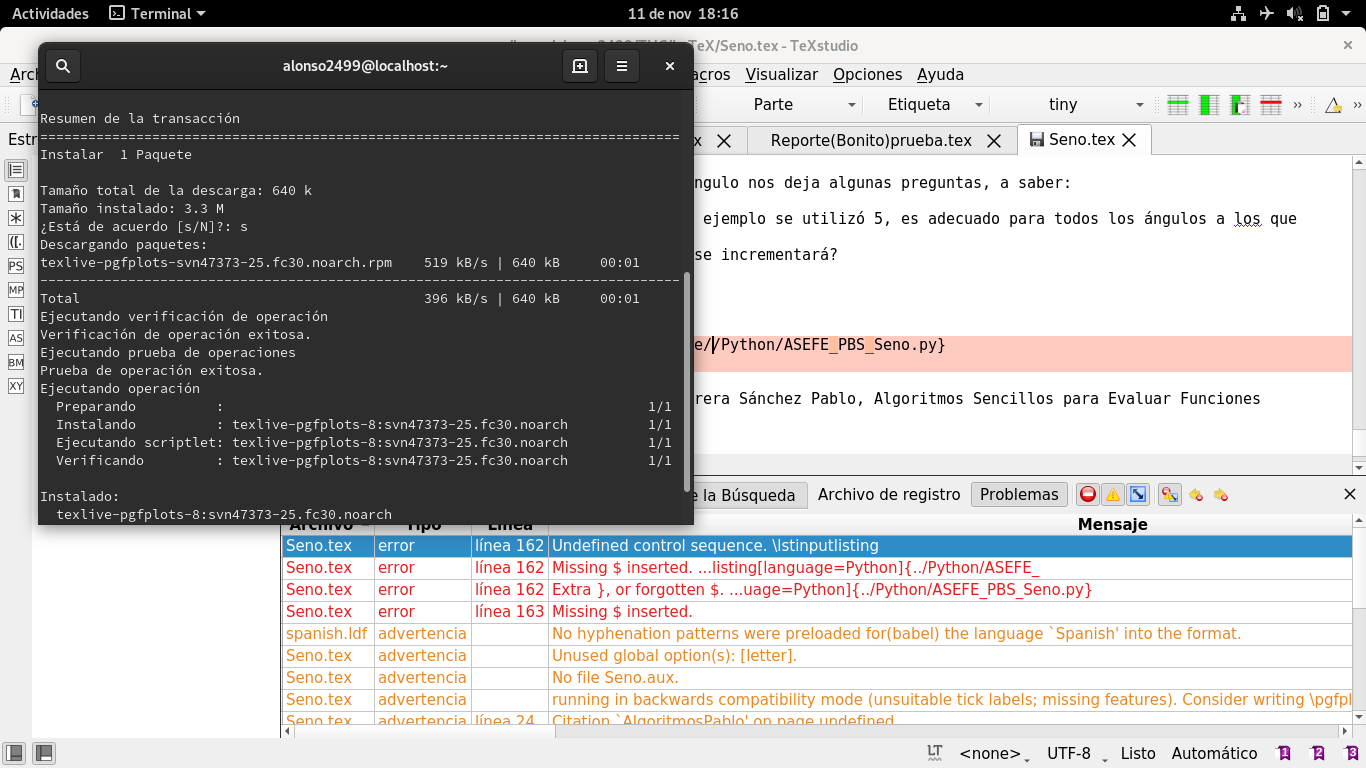
\includegraphics[scale=0.20]{/home/alonso2499/THC/LaTeX/Imagenes/ER3.png}

Pero después de esto me seguía mandando un error sobre una línea que comezaba con "lstinputlisting" así que recurrí a googlearlo y esto fue lo que encontré:

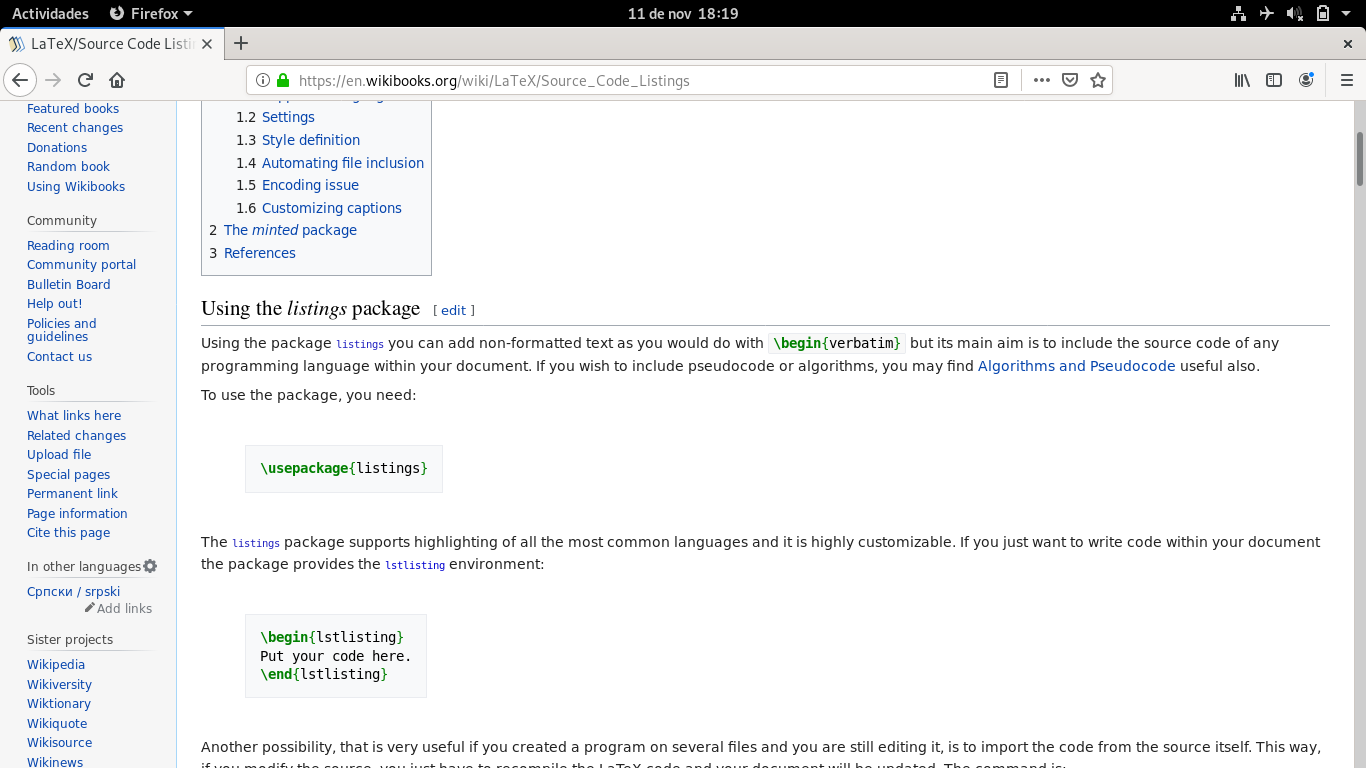
\includegraphics[scale=0.20]{/home/alonso2499/THC/LaTeX/Imagenes/ER2.png}

Sabiendo esto, recurrí a llamar la paquetería y a modificar la dirección que tenía esa línea y llevarla a un archivo que sabía que tenía y eso funcionó, ahora podía correr el archivo sin problema:

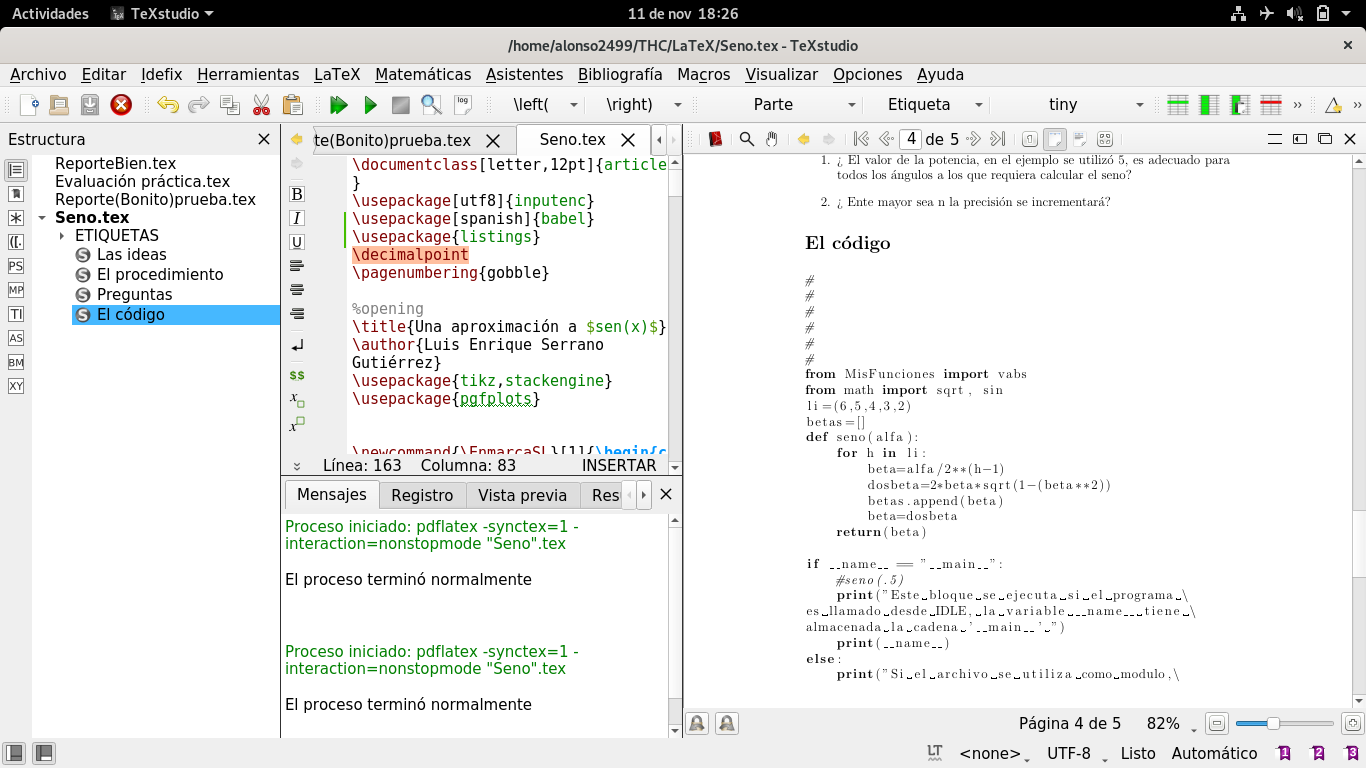
\includegraphics[scale=0.20]{/home/alonso2499/THC/LaTeX/Imagenes/ER1.png}

\end{document}
